\documentclass[../MLDM_Main.tex]{subfiles}

\begin{document}

\section{Knowledge Discovery and Data Mining Process (KDD)}
\textbf{Definition Data Mining:}\\
Process of discovering patterns in large data sets. Methods involved at the intersection of (machine learning, statistics and database systems.\\\\
\textbf{Goal of KDD:} Extract hidden, potentialy useful knowledge and actionable information from data.



\section{Machine Learning Paradigms}
\begin{itemize}
	\item Unsupervised learning (unlabeled)
	\item Supervised learning (labeled)
	\item Reinforcement learning
\end{itemize}

\subsection{Unsupervised Learning}
\paragraph{Clustering}
Grouping a set of objects in such a way that objects in the same group are more similar to each other than to those in other clusters.

\subsection{Supervised Learning}

\begin{figure}[H]
\centering
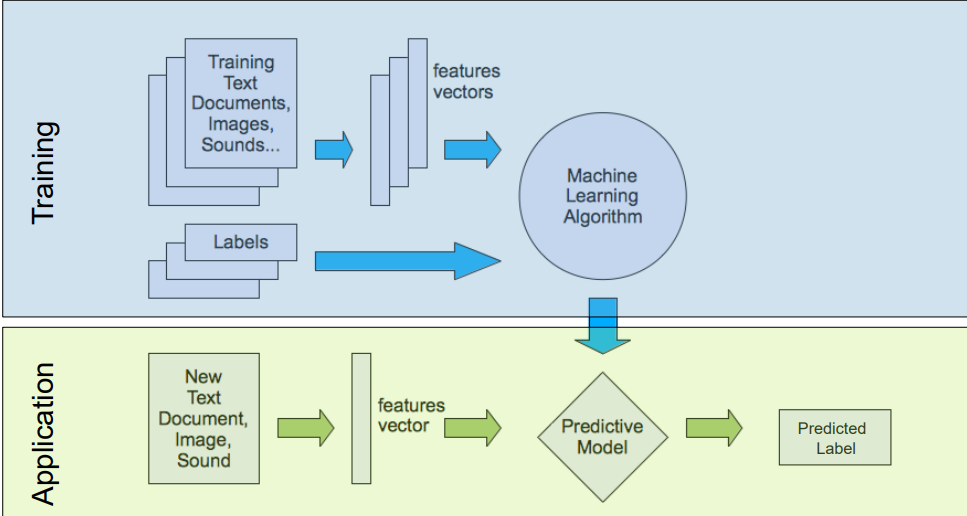
\includegraphics[width=0.3\textwidth]{images/SupervisedLearning.png}
\caption{\label{fig:Supervised Learning}Supervised Learning.}
\end{figure}
\paragraph{Example\\}
\textbf{Data:} Historic data from bank clients (Income, credit scores etc.)\\\textbf{Goal:} Forecast wheter a new client should be granted a loan or not.

\subsection{Reinforcement-Learning}
\begin{figure}[H]
\centering
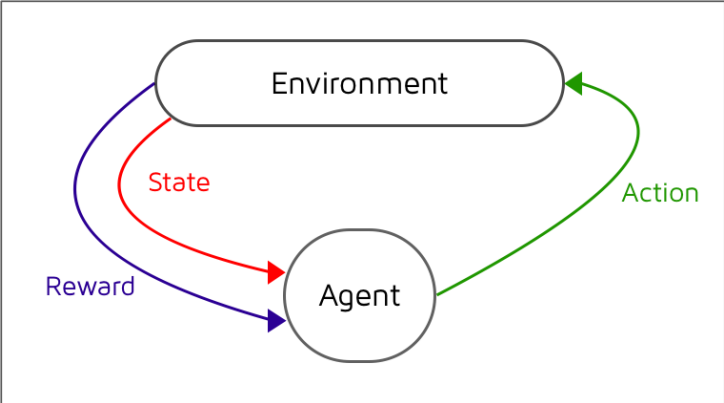
\includegraphics[width=0.3\textwidth]{images/ReinforcementLearning.png}
\caption{\label{fig:Reinforcement Learning}Reinforcement Learning.}
\end{figure}
\newpage
\subsection{Data}
\begin{itemize}
	\item \textbf{Data in Analaytics}
	\begin{itemize}
		\item \textcolor{red}{\textbf{Structured Data}}
		\begin{itemize}
			\item \textcolor{violet}{\textbf{Categorical}}
			\begin{itemize}
				\item Nominal
				\item Ordinal
			\end{itemize}
			\item \textcolor{violet}{\textbf{Numerical}}
			\begin{itemize}
				\item Continous
				\item Discrete
			\end{itemize}
			
		\end{itemize}				
		\item \textcolor{red}{\textbf{Unstructured or Semistructured Data}}
		\begin{itemize}
			\item \textcolor{violet}{\textbf{Textual}}
			\item \textcolor{violet}{\textbf{Multimedia}}
			\begin{itemize}
				\item Image
				\item Audio
				\item Video
			\end{itemize}
			\item \textcolor{violet}{\textbf{XML/JSON}}
		\end{itemize}
	\end{itemize}
\end{itemize}

\subsubsection{Data Classes}
\begin{itemize}
	\item One-Dimensional data
	\item Multi-Dimensional data
	\item Network data
	\item Hierarchical data
	\item Time-Series
	\item Geographic data
\end{itemize}

\section{Data Preprocessing}
\textbf{Tasks:}
\begin{itemize}
	\item Data Integration/consolidation
	\begin{itemize}
		\item Collects and merges data from multipe sources into a coherent data store
	\end{itemize}
	\item Data Cleaning
	\begin{itemize}
		\item Removing or modifying incorrect data, identify and reduce noise in data
	\end{itemize}
	\item Data transformations
		\begin{itemize}
			\item Normalize, discretize or aggregate the data
		\end{itemize}
	\item Data reduction
	\begin{itemize}
		\item Reduce data size by reducing the number of samples or reducing the number of attributes, balance skewed data
	\end{itemize}
	
\end{itemize}

\subsection{Data Cleaning}
\subsubsection{Detect (Near Duplicates)}
\textbf{For numeric values:}\\
\textcolor{magenta}{Cosine Similarity} of feature vectors\\
\textbf{For text:}\\
\textcolor{magenta}{Levensthein distance} between the texts\\
\subsubsection{Levensthein Distance}
Computes the minimum number of \textbf{Edit Operations} that are necessary to transform a word into another word.\\
\textbf{Operations:} Insert, Delete, Replace\\
\textbf{Runtime:} O(m*n) $->$ for 2 words of length m and n, with a dynamic programming algorithm

\subsubsection{Cosine Similiraty}
\textbf{Given:}\\
$A = \left(
	 \begin{array}{c}
	 a_1\\
	 a_2\\
	 .\\
	 .\\
	 .\\
	 a_n
	 \end{array}
	 \right)$ $B = \left(
	 \begin{array}{c}
	 b_1\\
	 b_2\\
	 .\\
	 .\\
	 .\\
	 b_n
	 \end{array}
	 \right)$\\\\

$cos(\theta) = \frac{A * B}{||A||*||B]]}$
\begin{figure}[H]
\centering
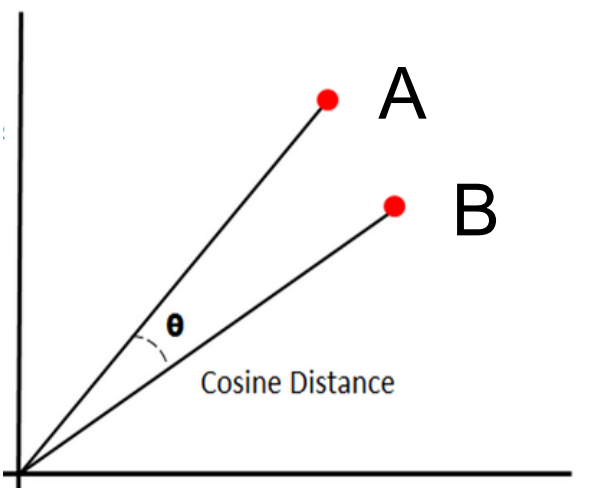
\includegraphics[width=0.3\textwidth]{images/CosineSimilarity.png}
\caption{\label{fig:Cosine Similarity}Cosine Similarity.}
\end{figure}
\subsubsection{Missing Values}
\begin{itemize}
	\item Interpolation
	\item Durchschnitt
	\item Regression
	\item Werte vordefinieren zum anwählen
\end{itemize}
\begin{figure}[H]
\centering
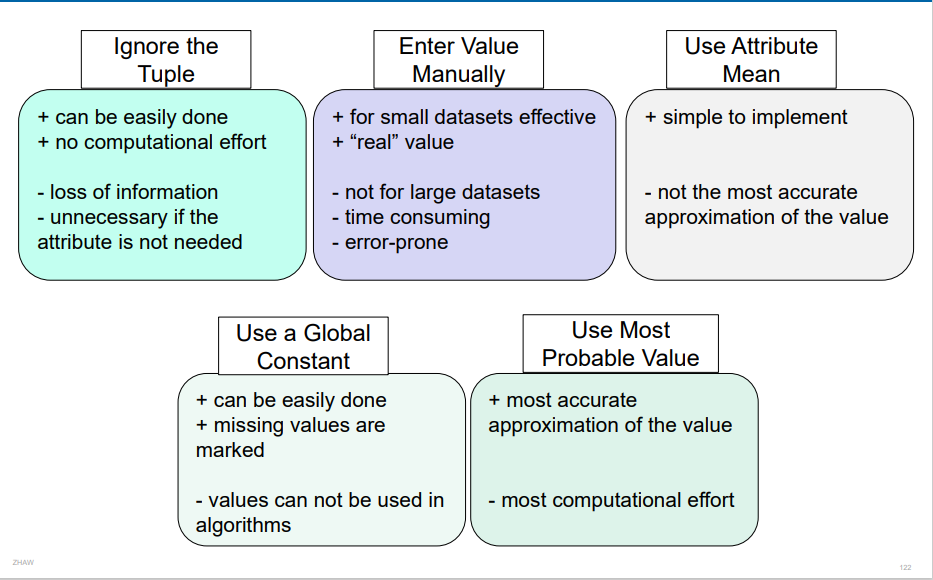
\includegraphics[width=0.3\textwidth]{images/MissingValues.png}
\caption{\label{fig:Missing Values}Missing Values.}
\end{figure}


\subsubsection{Outlier Detection}
Outlier Detection with Clustering (DBSCAN)

\subsubsection{Smoothing}
\textbf{Goal:} Make patterns \colorbox {yellow}{noticeable}, \colorbox {yellow}{eliminate disturbances} and outliers from data.\\
\textbf{Methods:}
\begin{itemize}
	\item Binning
	\item Regression
	\item Clustering
\end{itemize}


\subsubsection*{Binning}
\textbf{Equal-width Binning}\\\\
$Width = \frac{(max-min)}{N}$
\begin{itemize}
	\item N = number of intervals (Example N=3)
	\item  24, 28, 29, 35, 41, 41, 44, 45, 46, 48, 49, 54
	\item outliers may dominate result
	\item Width= 10
\end{itemize}

\begin{figure}[H]
\centering
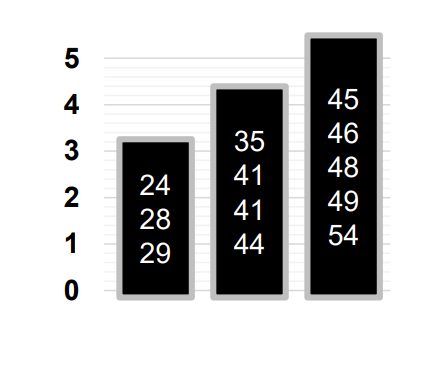
\includegraphics[width=0.3\textwidth]{images/EqualWidthBinning.png}
\caption{\label{fig:Equal-Width Binning}Equal-Width Binning.}
\end{figure}

\textbf{Equal-depth Binning}\\\\
$\frac{(Data amount)}{N}$
\begin{itemize}
	\item first sort Data
	\begin{itemize}
		\item 24, 28, 29, 35, 41, 41, 44, 45, 46, 48, 49, 54
	\end{itemize}
	\item N = number of intervals (example N=3)
	\begin{itemize}
		\item $[24, 28, 29, 35], [41, 41, 44, 45], [46, 48, 49, 54]$
	\end{itemize}
	\item outliers may dominate result
\end{itemize}
\colorbox {pink!60}{Smoothing by bin means:}
Replace each value by the mean value of the bin\\$[29, 29, 29, 29], [43, 43, 43, 43], [49, 49, 49, 49]$\\\\
\colorbox {pink!60}{Smoothing by bin boundaries:}
Replace each value by closest boundary value\\$[24, 24, 24, 35], [41, 41, 45, 45], [46, 46, 46, 54] $

\subsection{Data Transformation}
\textbf{Discretization:} Convert continous variables to discrete using binning\\\\
\textbf{Aggregation:} Reduce the number of categories for categorical variables applying proper concept hierarchies\\\\
\textbf{Construct new features:} Derive new, potentially more informative feature from the existing ones using different mathematical functions (e.g. multiplication)

\section{Feature Scaling}
\textbf{Problem:} Features have different values (e.g weights between 70-100kg vs height between 1.6-20m)\\\\
\textbf{Goal:} Make all features (columns of X) approximateley of equal size typically around zero





\end{document}
